\documentclass{article}
\usepackage[utf8]{inputenc}
\usepackage{amsmath}
\usepackage{graphicx}
 \usepackage{listings}
\usepackage[top=1.55cm, bottom=2.29cm, left=1.6cm, right=1.47cm]{geometry}

% This is for the fancy title in each page
\usepackage{fancyhdr}
\lhead{}
\chead{}
\rhead{First Session: Combinational Design}
\pagestyle{fancy}

\usepackage{enumitem}


\makeatletter
\def\threedigits#1{\expandafter\@threedigits\csname c@#1\endcsname}
\def\@threedigits#1{%
  \ifnum#1<100 0\fi
  \ifnum#1<10 0\fi
  \number#1}
\makeatother
\AddEnumerateCounter{\threedigits}{\@threedigits}{100}


%\setenumerate[1]{}


\begin{document}

%%%% FRONTPAGE %%%%%%%%%%%%%%%%%%%%%%%%%%%%%%%%%%%%%%%%%%%%%%%%%%%%%%%%%%%
\begin{titlepage}

\begin{center}
%
\includegraphics[width=0.25\textwidth]{./uc3m.jpg}\\[2cm]
\textsc{\huge Bachelor's Thesis:\\[0.5cm]In-hand object detection and tracking using\\[0.5cm]2D and 3D
information }\\[4cm]


% Title
{\Huge\bfseries{Software Requirements Specification}\\[2cm]}

\Large{Version 0.2}
\\[11cm]


% Author and supervisor
\begin{minipage}{0.55\textwidth}
\begin{flushleft} \large
\emph{Author:}\\
Irene Sanz Nieto\\
\end{flushleft}
\end{minipage}
\begin{minipage}{0.4\textwidth}
\begin{flushright} \large
\emph{Supervisor:}\\
Victor González Pacheco\end{flushright}\end{minipage}\vfill

% Bottom of the page
{\large \today}

\end{center}
\end{titlepage}

%
\newpage
%
%%%%%%Table of contents%%%%%%%%%%%%%%%%%%%%%%%%%%%%%%
%%%%%%%%%%%%%%%%%%%%%%%%%%%%%%%%%%%%%%%%%%%%%%%%%%%%%
\tableofcontents
\newpage


%%%%%%Document%%%%%%%%%%%%%%%%%%%%%%%%%%%%%%%%%%
%%%%%%%%%%%%%%%%%%%%%%%%%%%%%%%%%%%%%%%%%%%%%%%%%%%%%
\section{Introduction}
\hspace{0.5cm}The project consists on an in-hand object learning and recognition software. 
%
\includegraphics[width=0.25\textwidth]{./uc3m.jpg}\\[2cm]
\subsection{Nodes}

\subsubsection{Event Handler Node}
	This node will identify the different user's gestures and act accordingly using a State Machine structure. 
	\begin{center}
		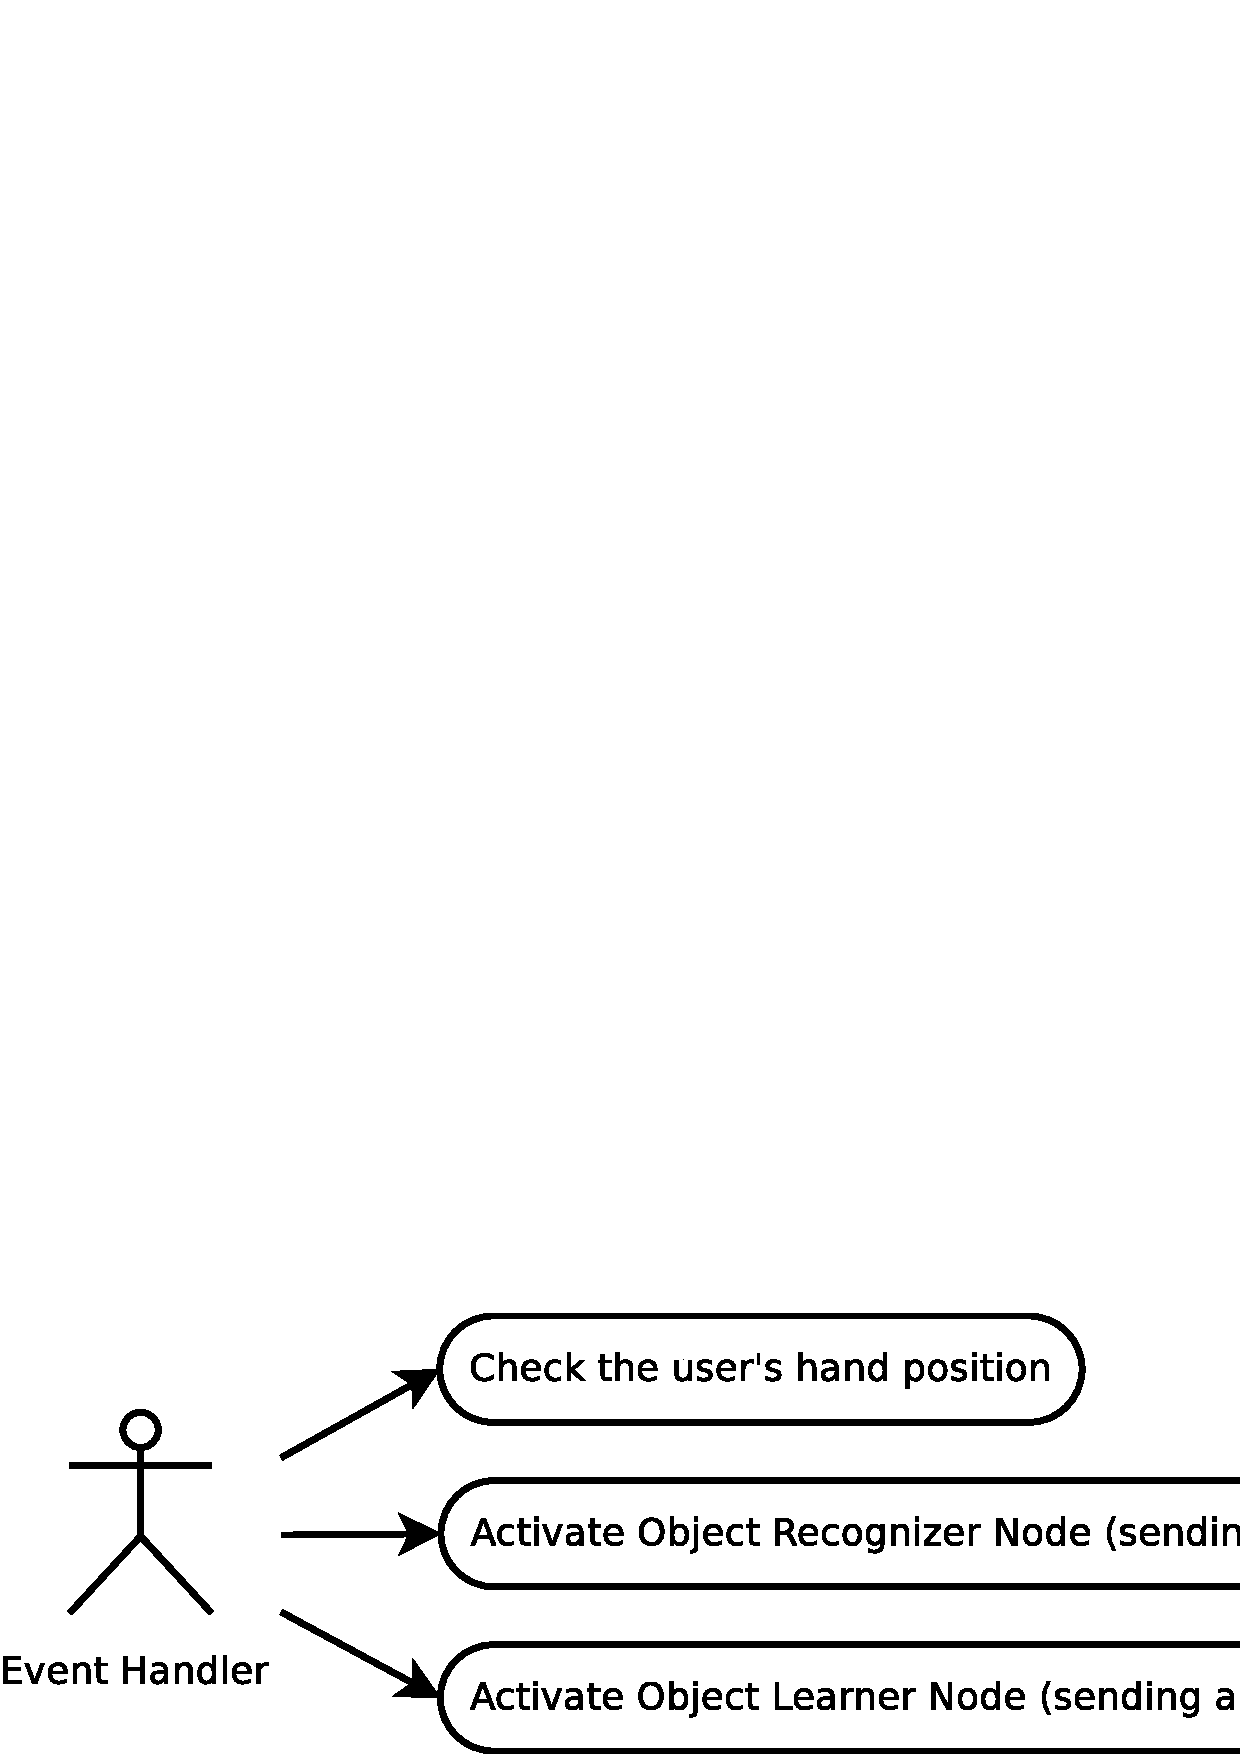
\includegraphics[scale=0.4]{../diagrams/images/uc_event_handler.jpeg}
	\end{center}
	
\subsubsection{Display Node}
This node will show the output of the program. There will be a window in which different informations will be shown. 
	\begin{center}
		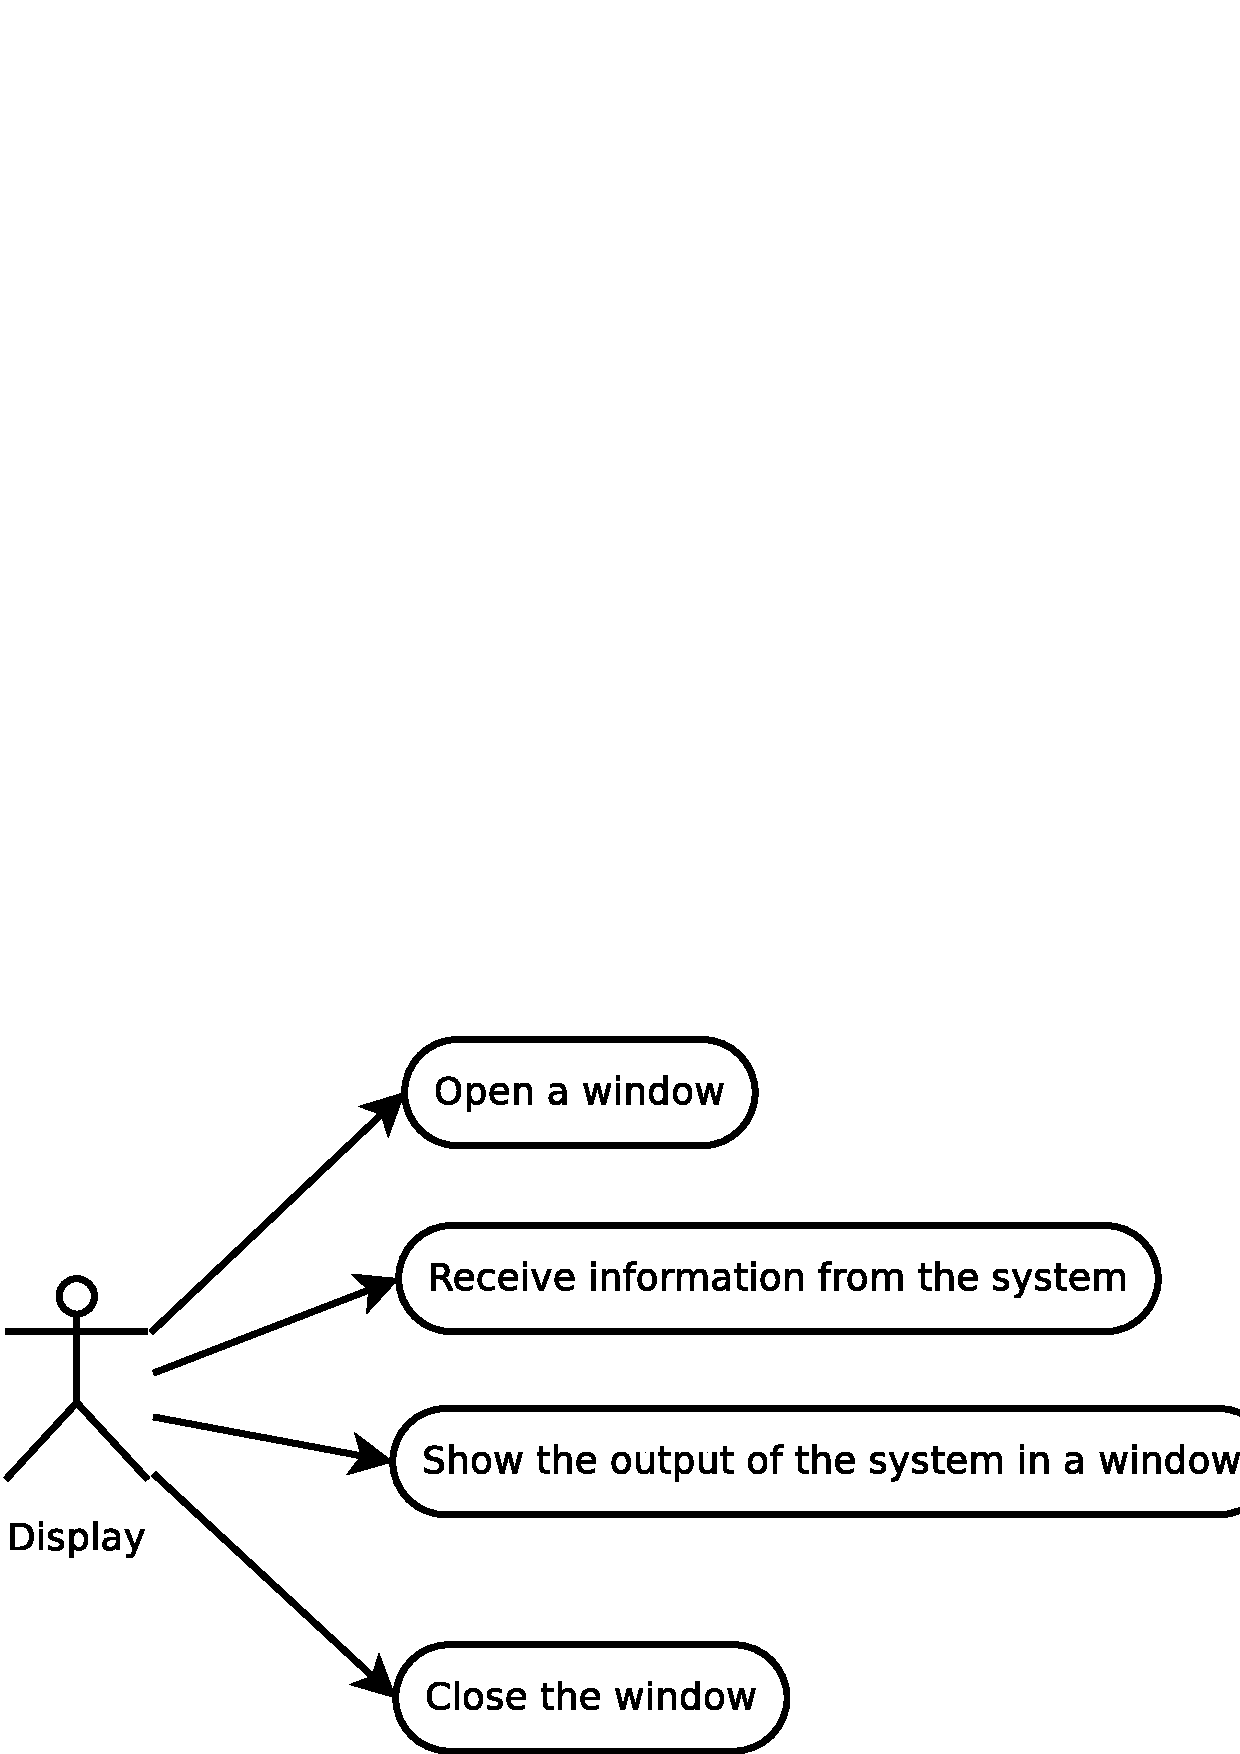
\includegraphics[scale=0.4]{../diagrams/images/uc_display.jpeg}
	\end{center}
	
\subsubsection{Object Learner Node}

\hspace{0.5cm}This node will learn new handheld objects. 

The sequence of the object learning is the following:
\\
First, 3D and 2D information will be extracted and written to a file. Then, two algorithms will be trained (one for 2D and the other for the 3D template). The parameters of each trained algorithm will be stored in a file. There will be hence one file per learned object and one file per algorithm.
\\

The learning of the objects will be done in-hand. This will allow a more intuitive interaction human-robot. The triggering of the learning mode will be to extend the hand in front of the body, showing the new object to the RGB-D sensor. When the user returns the arm to a position which is closer to the body, the algorithm will start learning the new object and after the learning, it will come back to the recognizing mode, which is the default. 

\begin{center}

		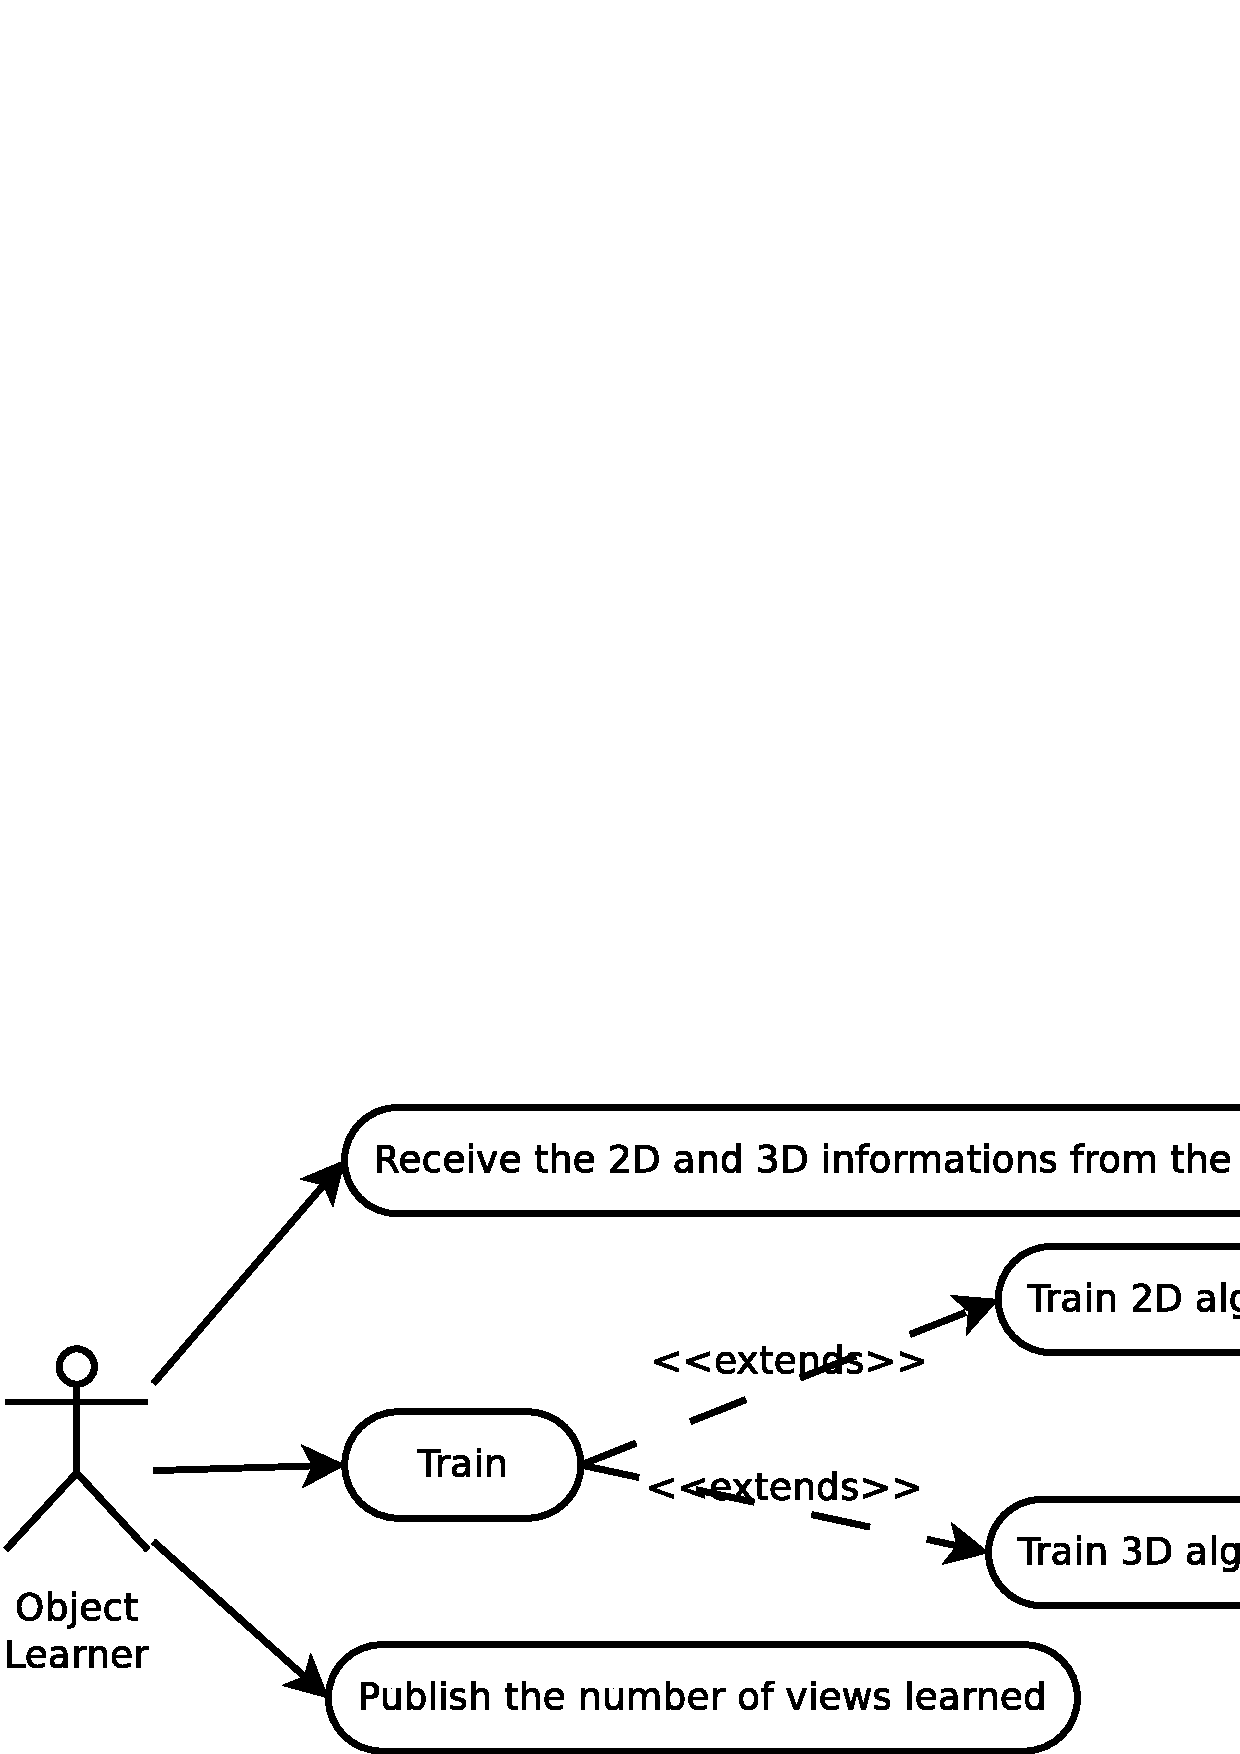
\includegraphics[scale=0.4]{../diagrams/images/uc_learner.jpeg}
	\end{center}

\subsubsection{Object Recognizer Node} 
\hspace{0.5cm}This node will track the user's hands and recognize the held objects. 

As in the Learning Mode, 2D and 3D information will be extracted. Then, the algorithms will compare that information with the learned one. Weights for each algorithm will be given, since each of them identifies a different characteristic. Finally, the name of the object will be shown on the screen. 

\begin{center}
	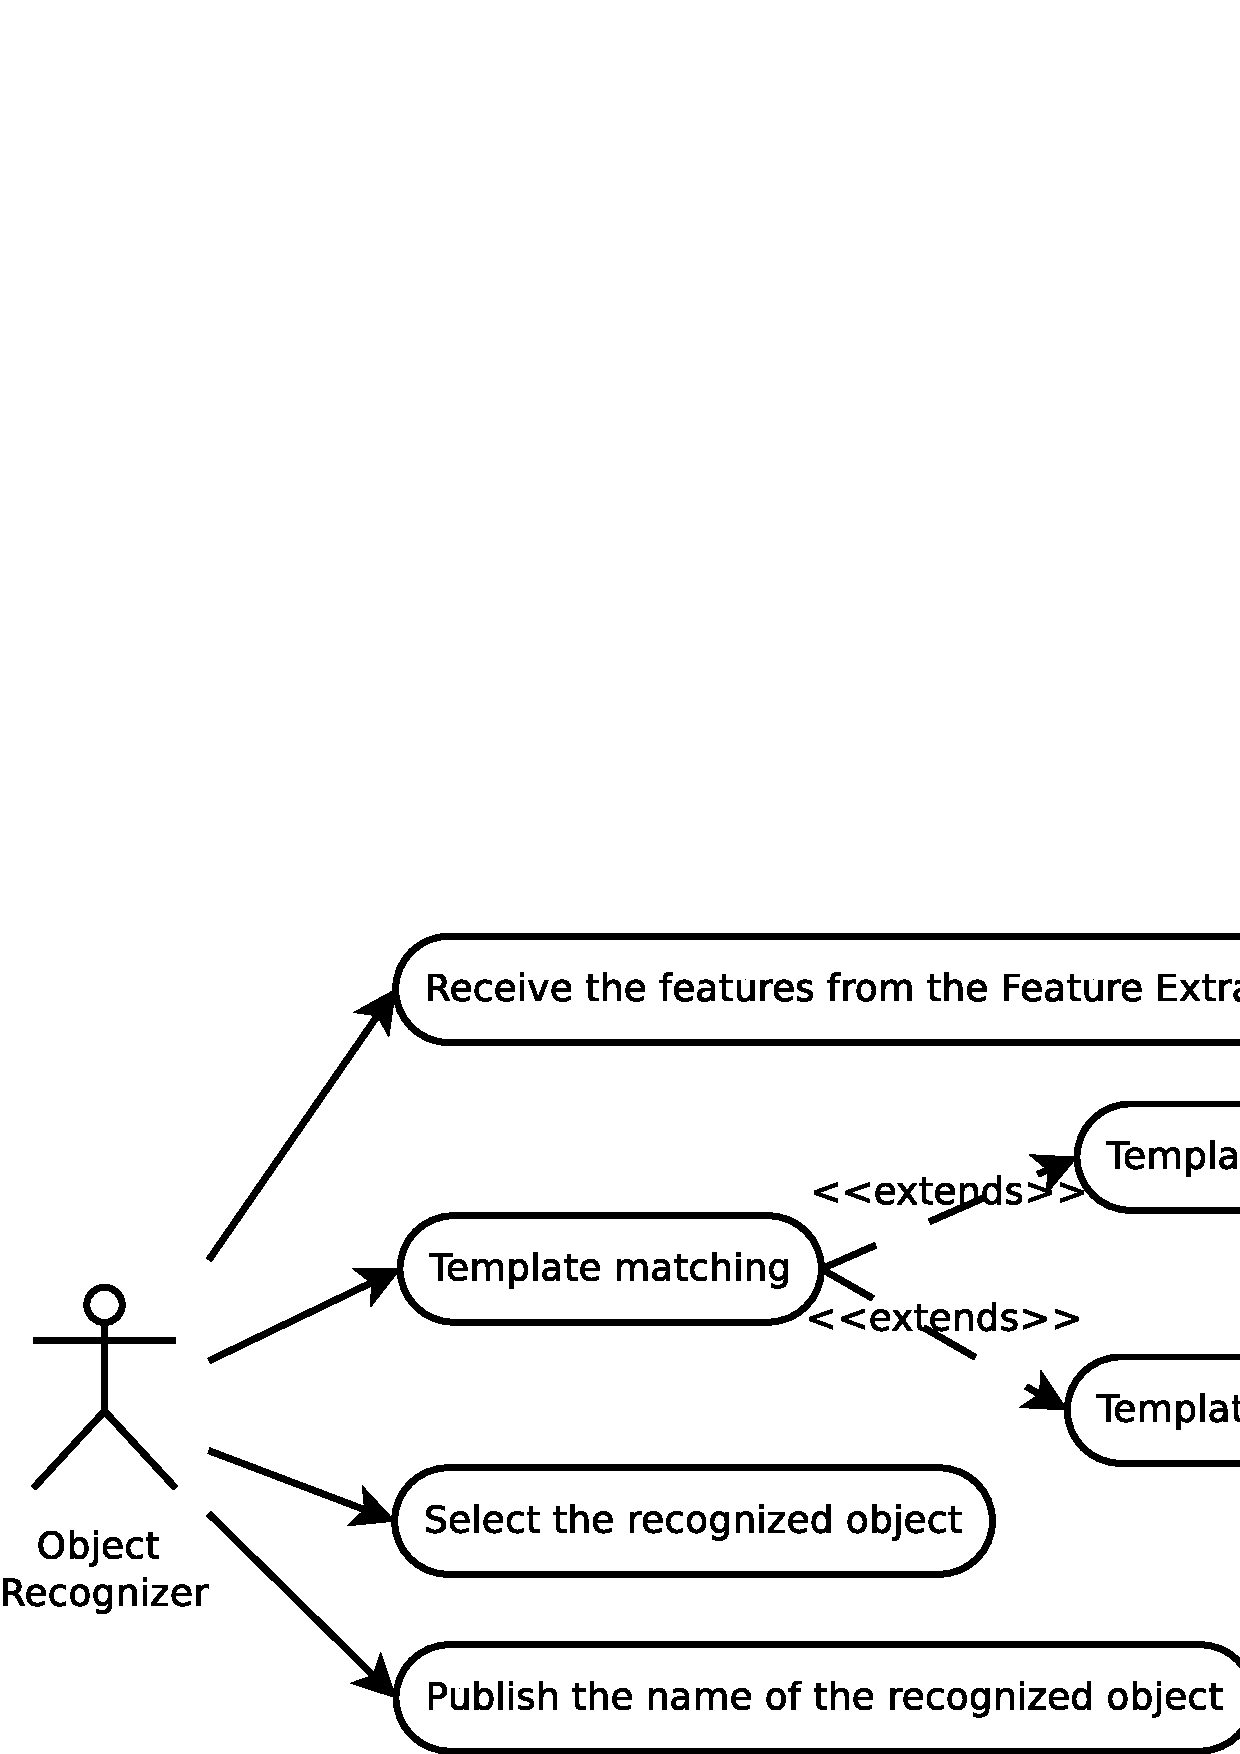
\includegraphics[scale=0.4]{../diagrams/images/uc_recognizer.jpeg}
\end{center}

\subsubsection{Converter Node}

This node will convert the messages from other ROS packages to the internal message format used within the code. 

\begin{center}
	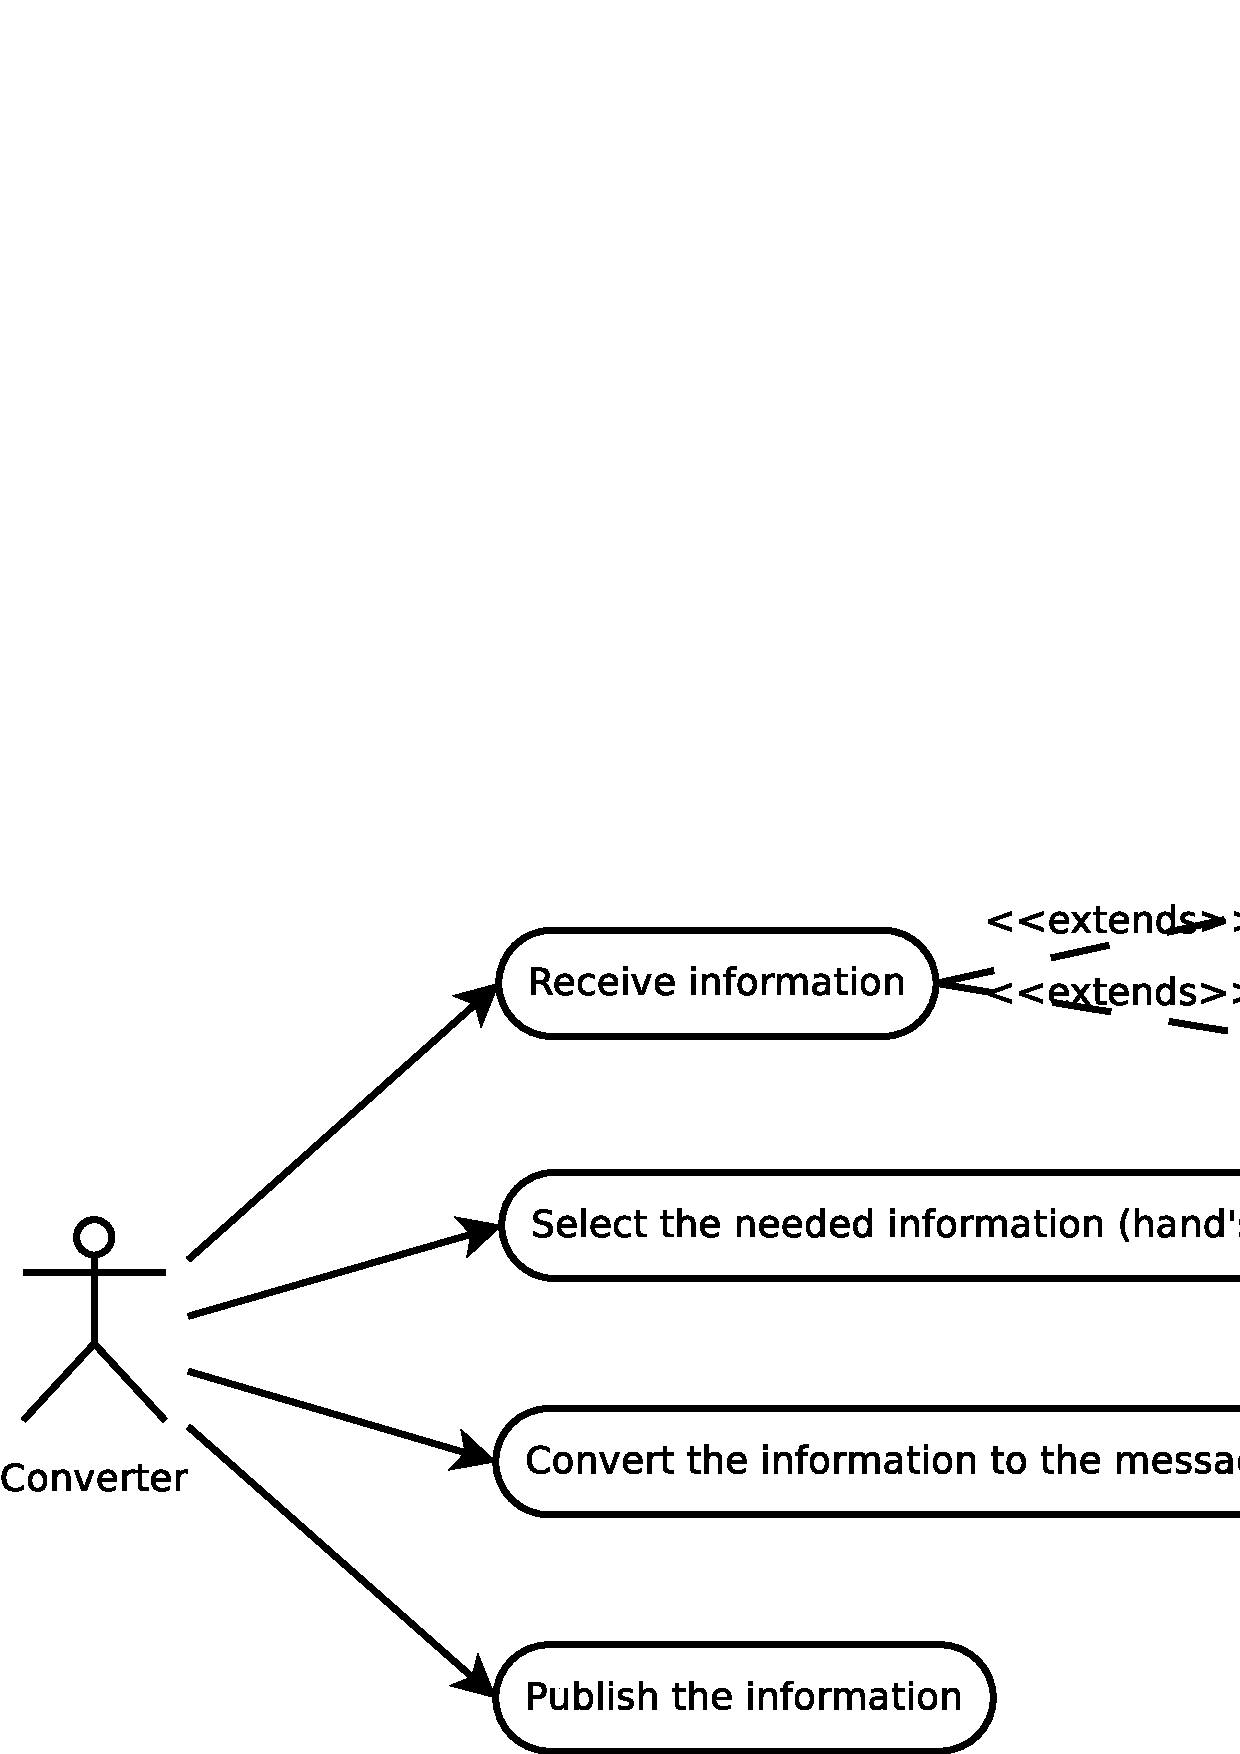
\includegraphics[scale=0.4]{../diagrams/images/uc_converter.jpeg}
\end{center}
	
\subsubsection{ROI Segmenter Node}
This node will segment the ROI (Region Of Interest) both in 2D and 3D.

\begin{center}
	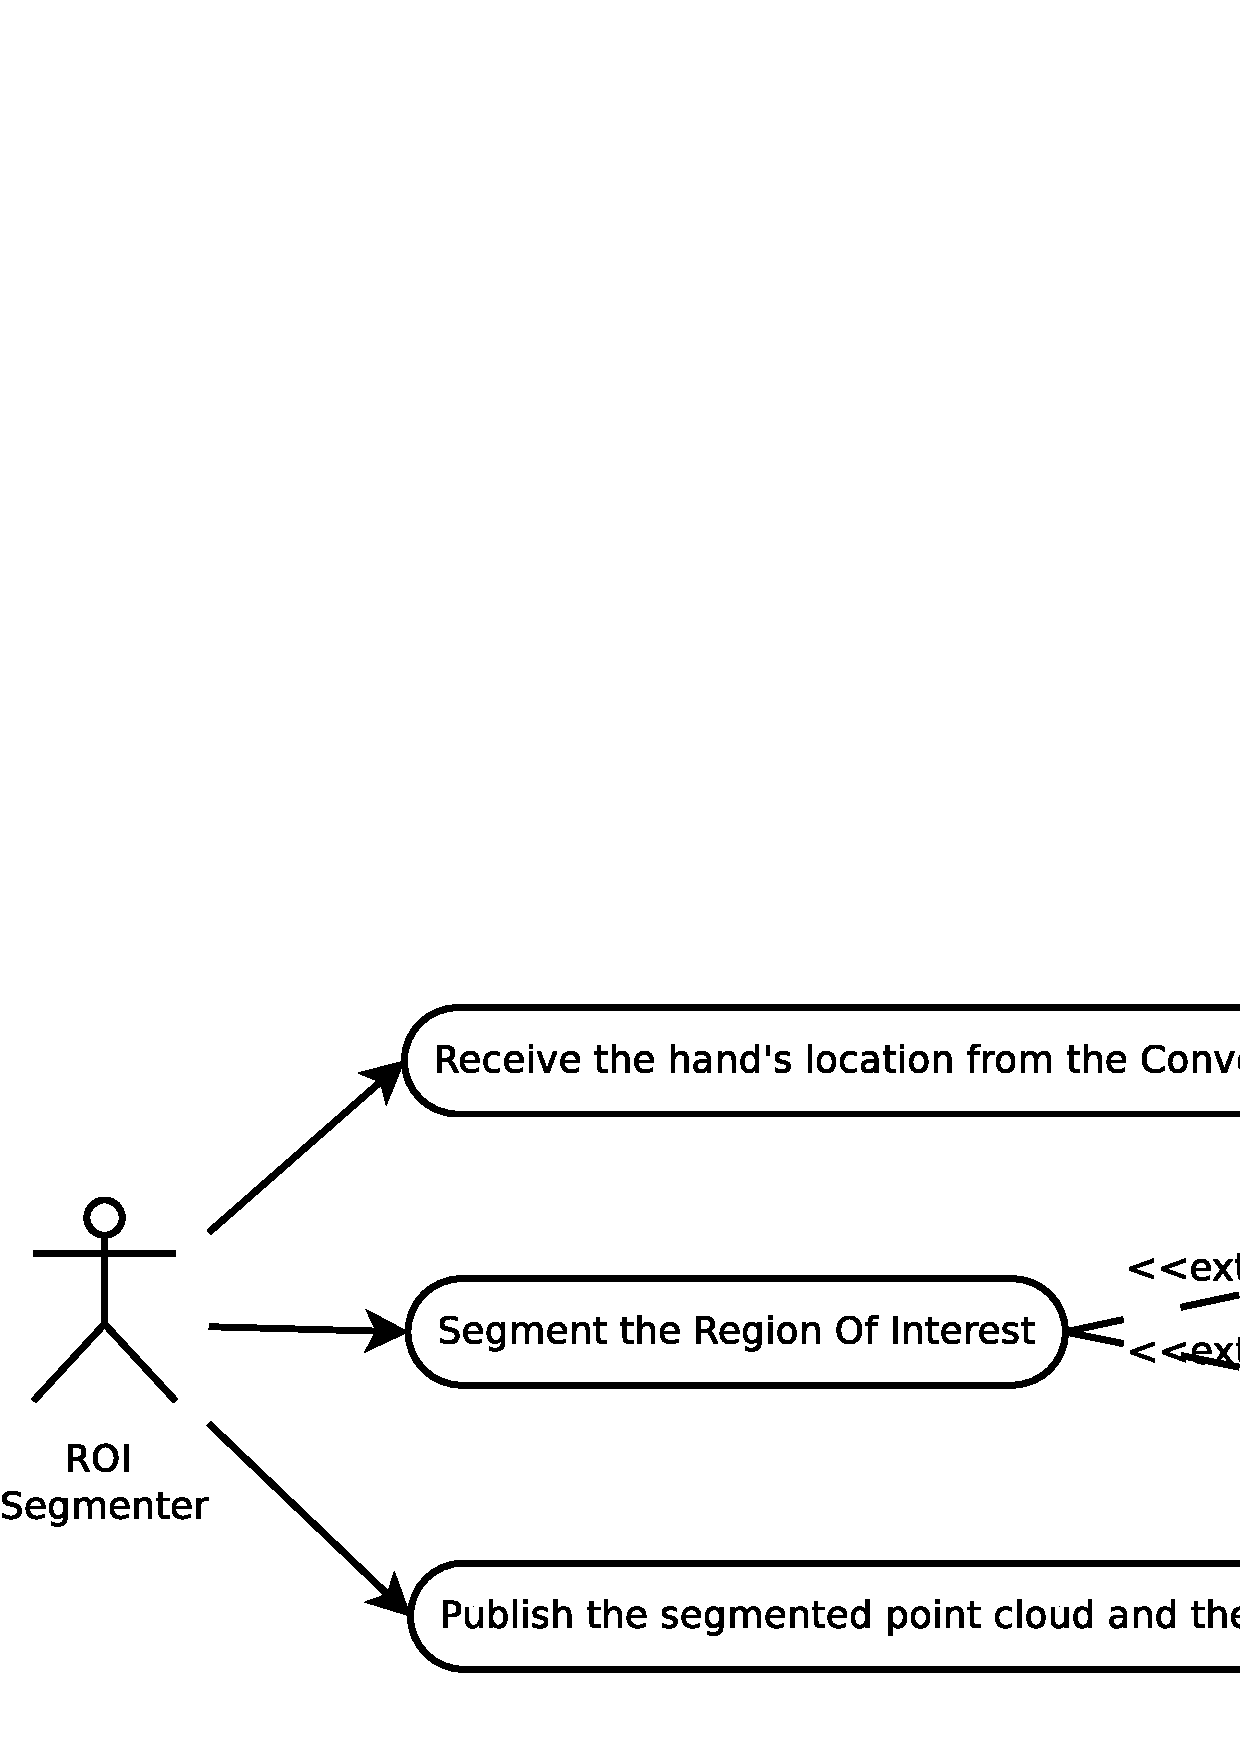
\includegraphics[scale=0.4]{../diagrams/images/uc_roi_segmenter.jpeg}
\end{center}

\subsubsection{Feature Extractor Node}
This node will extract both 2D and 3D features and publish them. 

\begin{center}
	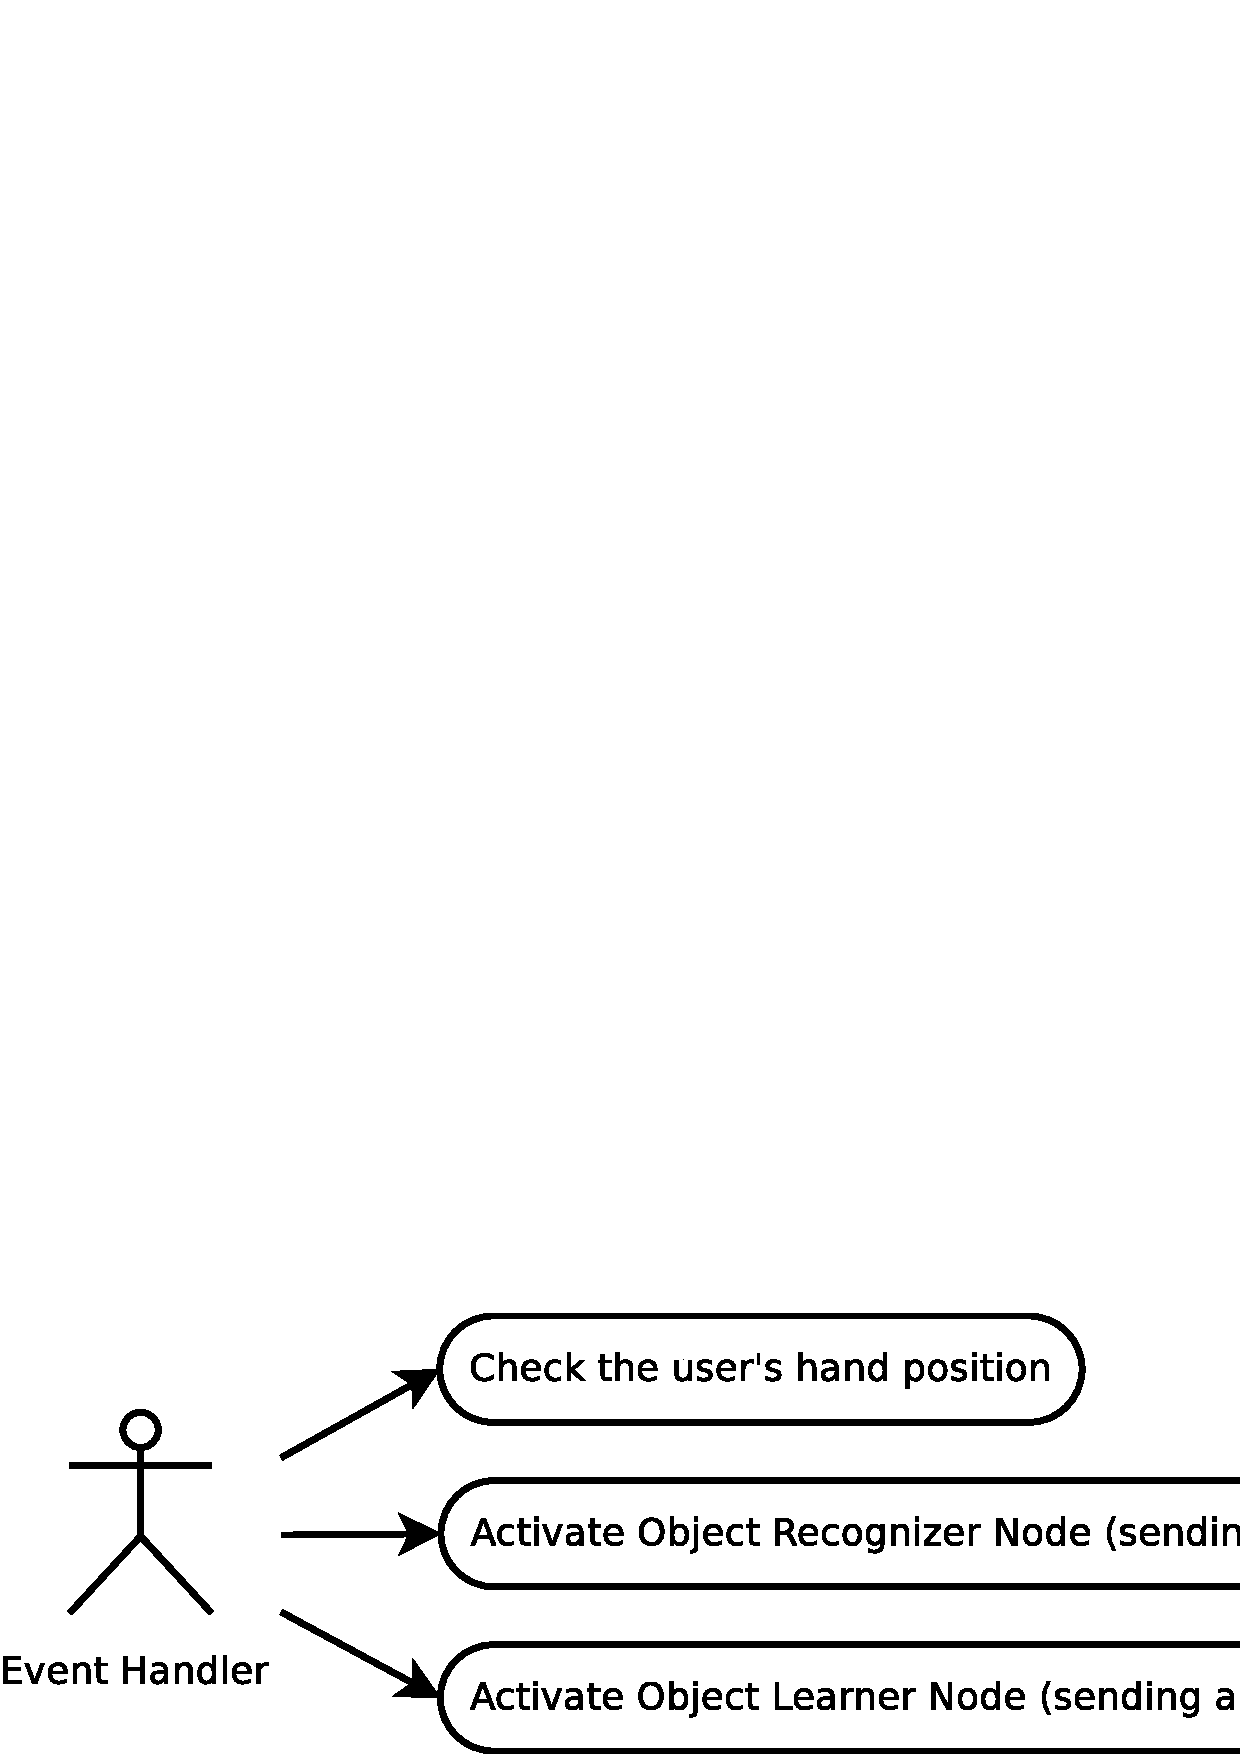
\includegraphics[scale=0.4]{../diagrams/images/uc_event_handler.jpeg}
\end{center}


\subsubsection{Data Parser Node}
This node will store the 2D and 3D features of each template of the same object in one file. 
\begin{center}
	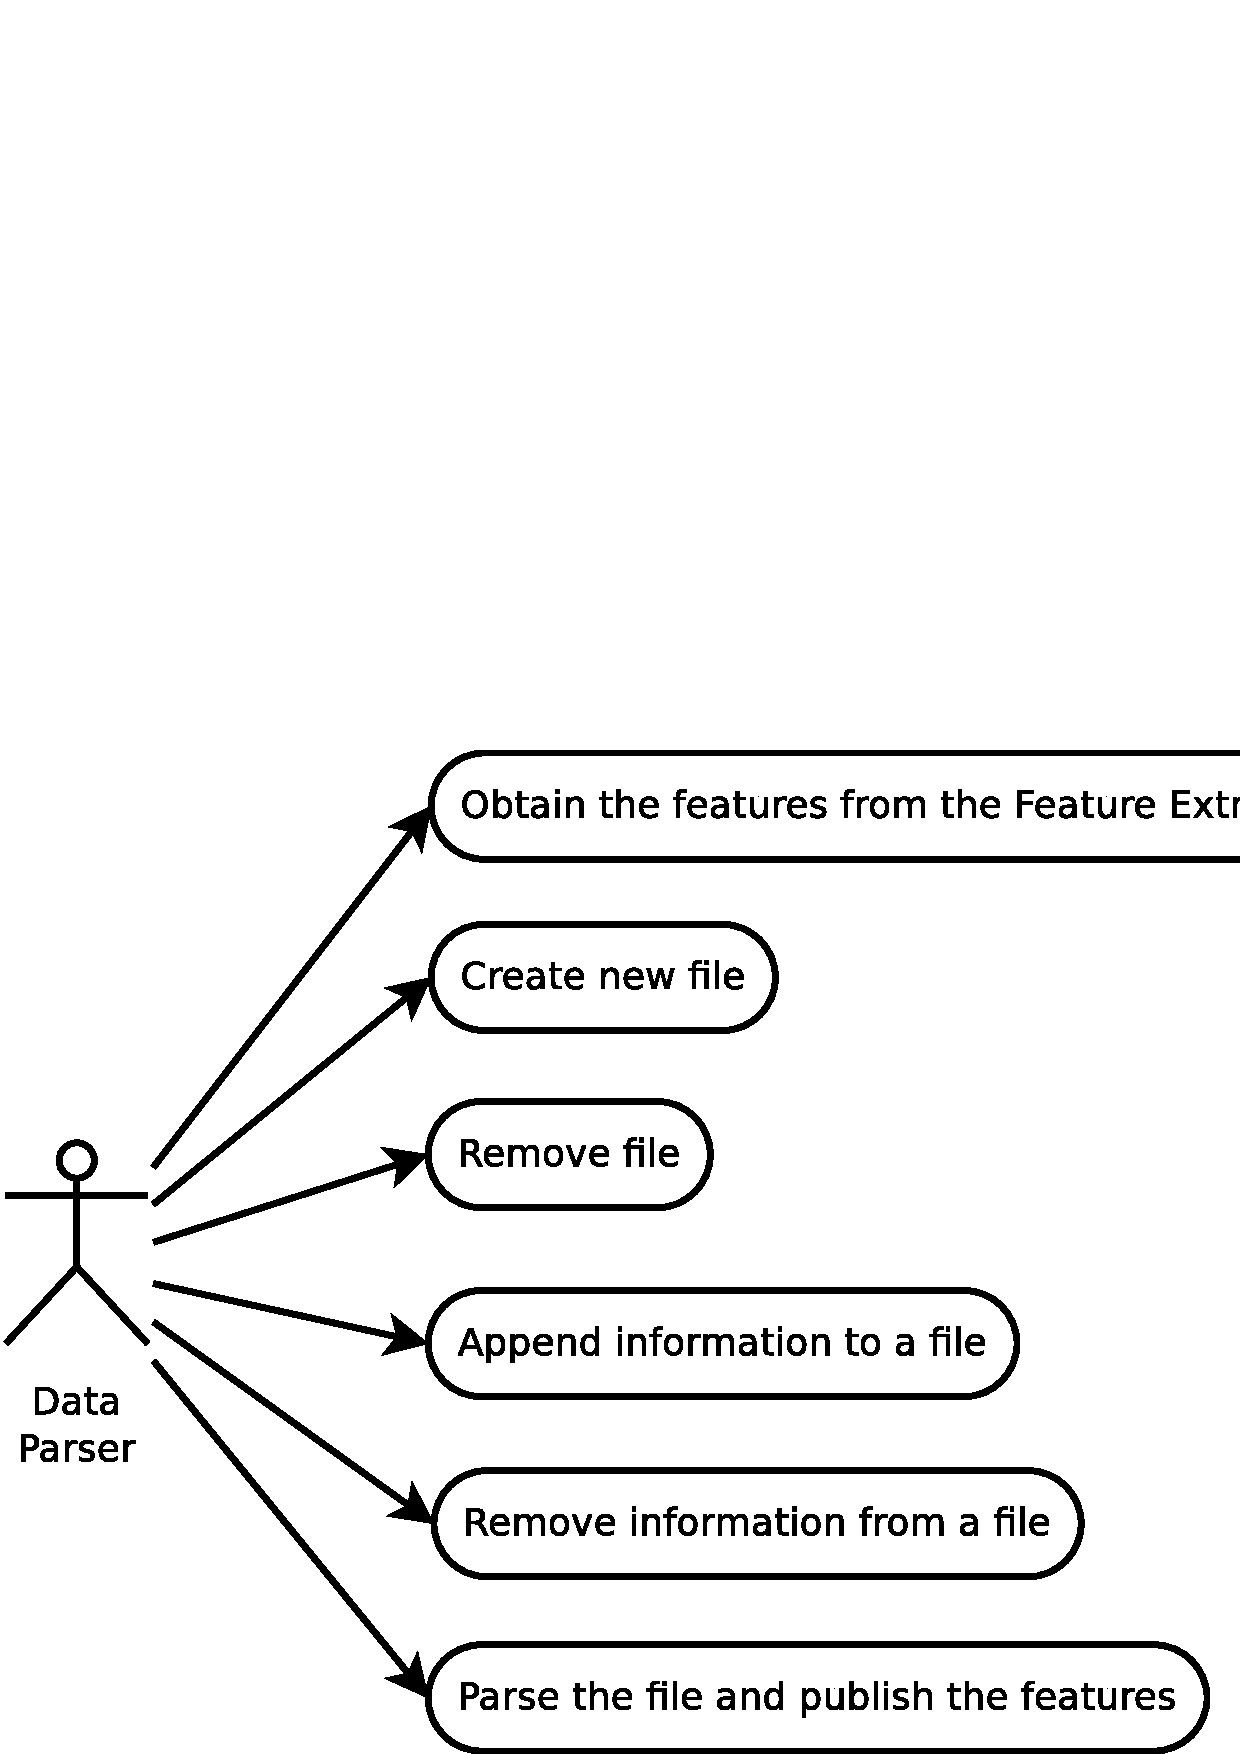
\includegraphics[scale=0.4]{../diagrams/images/uc_data_parser.jpeg}
\end{center}


\subsection{Third Party Packages}
\hspace{0.5cm}Initially only one third party ROS package will be used, to track the hand's position: pi\_ tracker. This software publishes the hand's position and there will a node in the proposed software (Conversion Node, whose requirements are specified in the next section) that converts the information returned by pi\_ tracker to the custom message used in the rest of the code.  

\subsection{Node Interaction}
In the following diagram it can be seen the interaction and the information exchanged between nodes.
\subsubsection{Use Case Diagram}
\begin{center}
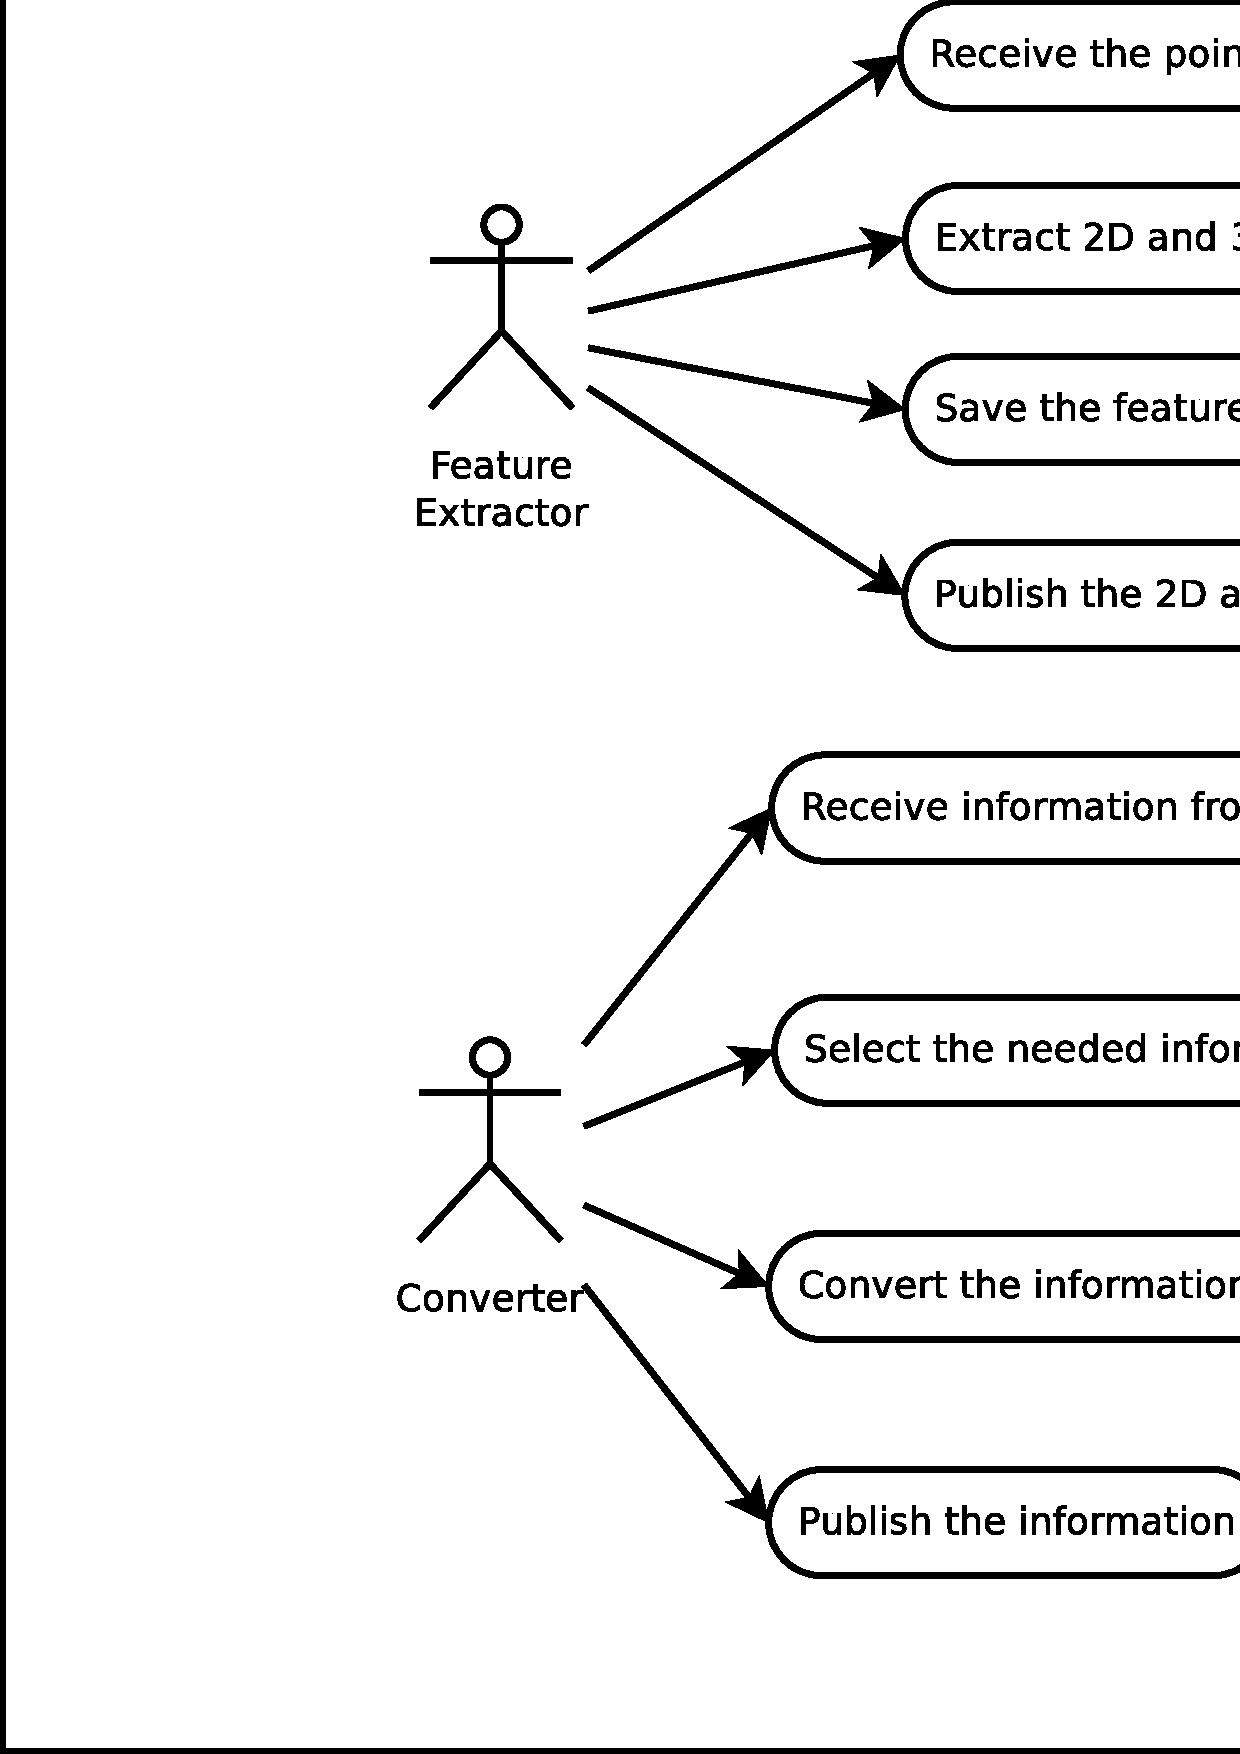
\includegraphics[scale=0.3]{../diagrams/images/use_case.jpeg}
\end{center}

\subsubsection{Sequence Diagram}
In the following diagram it can be seen the sequencial interaction between nodes. 
\begin{center}
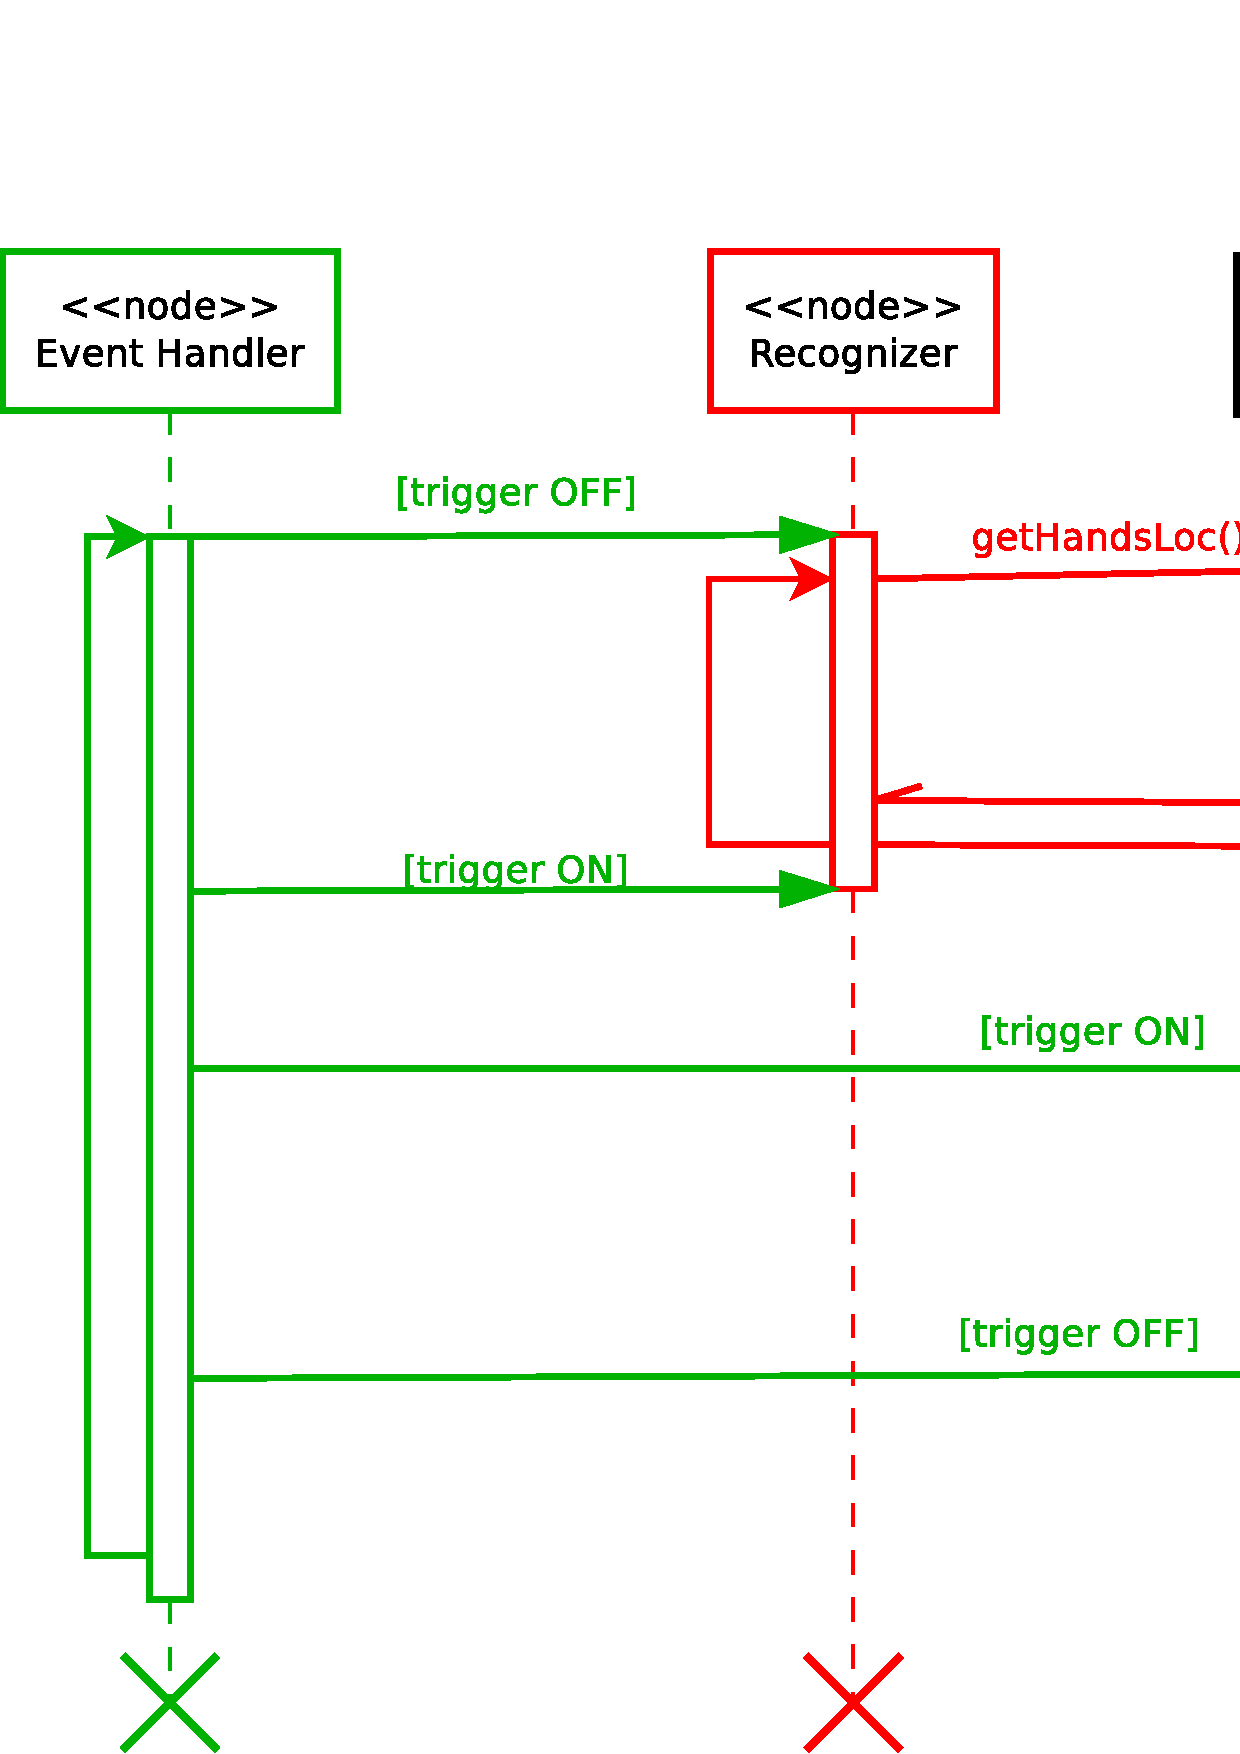
\includegraphics[scale=0.4]{../diagrams/images/sequence.jpeg}
\end{center}

\subsection{Flowchart}
In the following diagram, the flow of the program is represented. 
\begin{center}
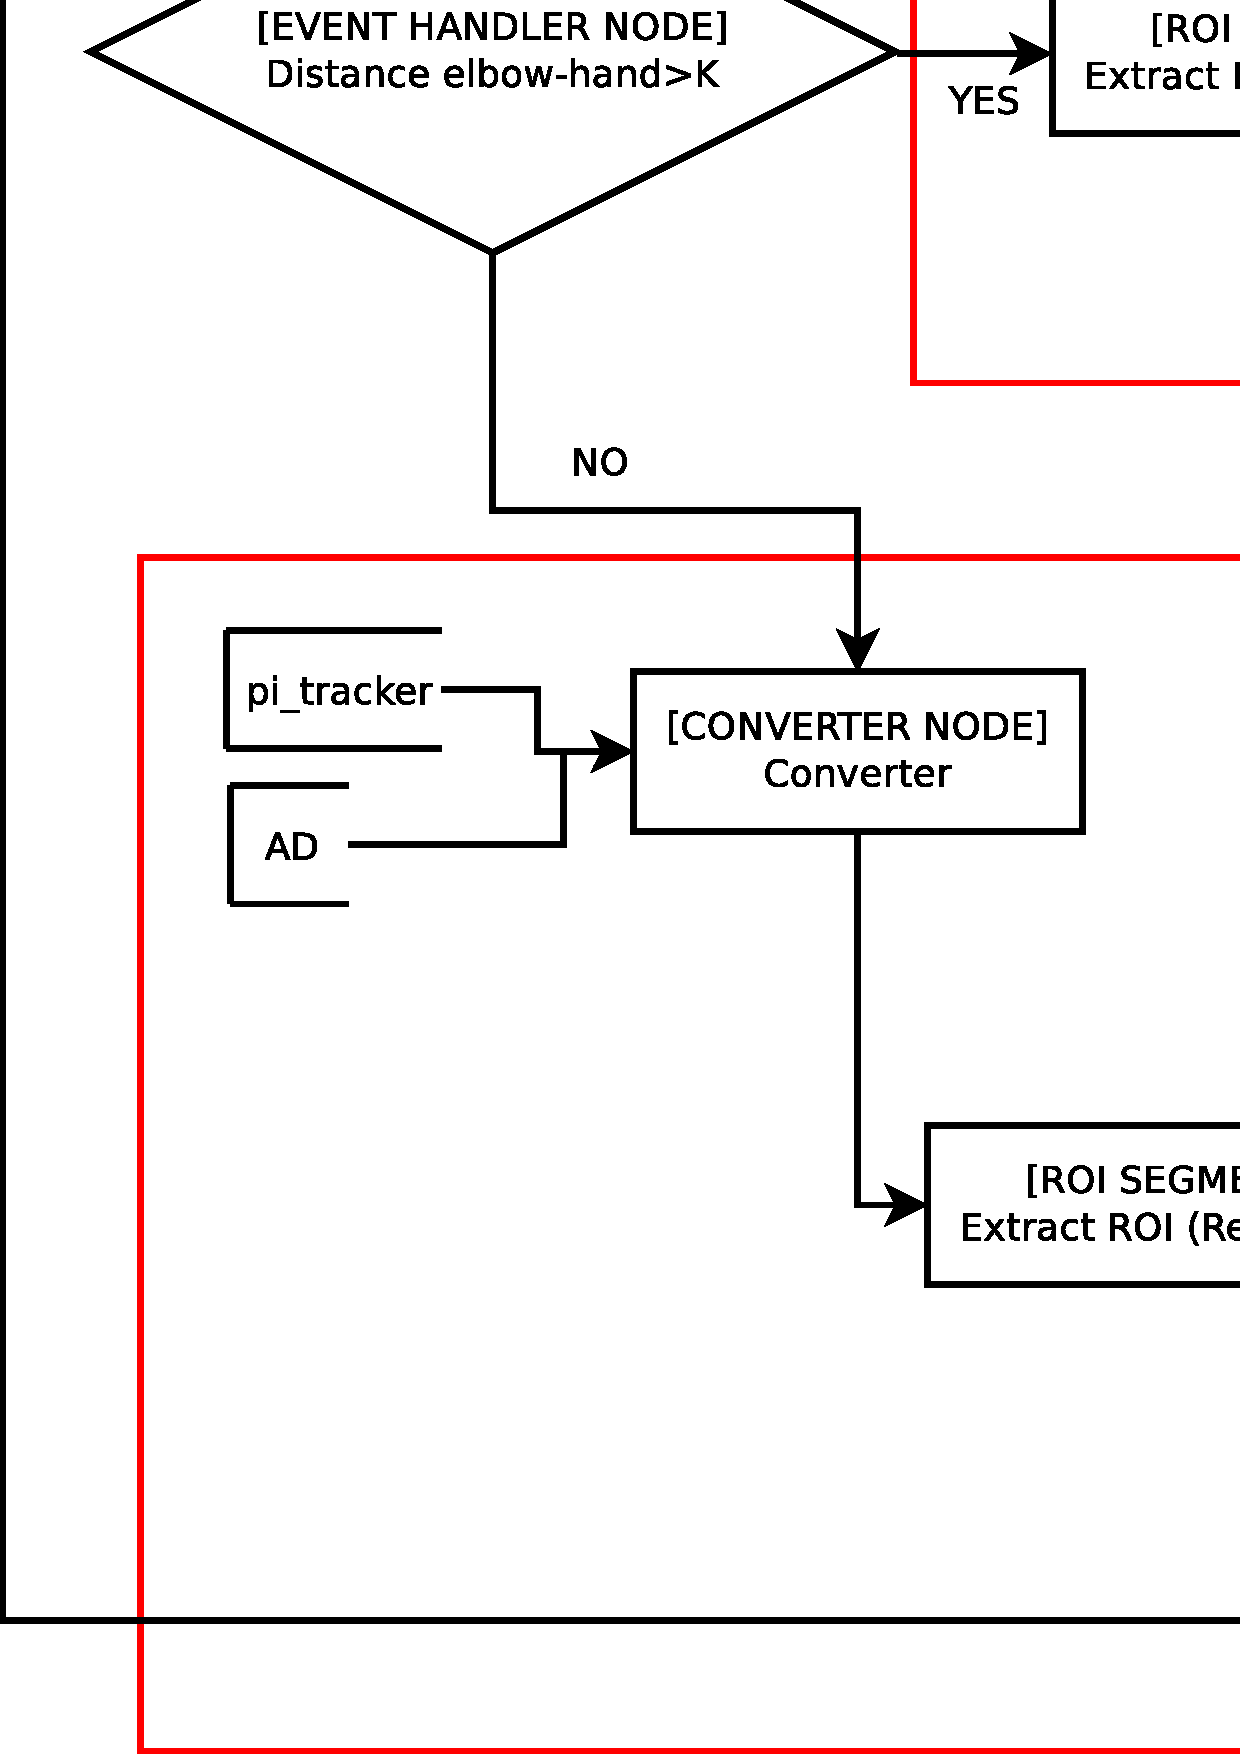
\includegraphics[scale=0.35]{../diagrams/images/flowcharts.jpeg}
\end{center}





\section{Functional requirements}

\subsection{General requirements}
\begin{enumerate}[label=\textbf{FR\threedigits*}]

	\item The software must be developed under ROS (Robotic Operating System), using the Groovy distro and rosbuild.
	\item A version control system should be used (GIT) and all the code must be periodically updated in the following github repository:  $https://github.com/irenesanznieto/TFG$
	\item The software hast to have an interface. Its requirements are specified in the following "Interface Requirements" section. 
	\item The software must accept as inputs the following RGB-D sensors: Microsoft Kinect, ASUS Xtion PRO, ASUS Xtion PRO Live, PrimeSense PSDK 5.0.
	\item The output of the system must be a node specifying the name of the detected object. 
 
\subsection{Event Handler}
 
\subsection{Display}

\item The program must have one window with the output of the camera of the kinect sensor. 
\item The information as to what mode the program is in hast to be shown in the title of the window.
\item In the recognition mode, the interface must show a square around the detected object and a text label indicating the object's name. Also, two points must be drawn in each of the hands. 
\item The learning mode should open a new window where an shpere will appear. The sphere must show a different colour when a template of that zone is made. On the main window, a square should be placed around the new object. 


\subsection{Object Learner}
	\item This node must have two algorithms, one for 2D and other for 3D. 
	\item The algorithm used with 2D features should be a BruteForce trainer.
	\item The algorithm used with 3D features will be the Line-Mod trainer. 	
	\item This node must send feedback messages to the display with the learning information (percentage of learning of the object, number of views of the object). 

\subsection{Object Recognizer}
	\item This node must have two algorithms, one for 2D and other for 3D. 
	\item The algorithm used with 2D features should be a BruteForce matcher.
	\item The algorithm used with 3D features will be the Line-Mod matcher. 
	\item A weighting must be made to the output of the matching process. This will help reduce the false positives and negatives by modelling occlusions depending on the hand-elbow relative positions. 
	\item A weighting must be made depending on the amount of texture possessed by each object to decide which matching should have more importance, the 2D or the 3D one. 



\subsection{Converter}

\item The information should be received subscribing to the topics of the different third-party packages. 
\item The internal message format must have the following structure: \\[0.3cm]
\textit{
std\_ msgs/Header header\\[0.1cm]
int32 id\\[0.1cm]
geometry\_ msgs/Vector3[] position\\
\hspace*{0.5cm}float64 x\\
\hspace*{0.5cm}float64 y\\
\hspace*{0.5cm}float64 z\\
}


\subsection{ROI Segmenter}
	\item This node will segment the Region Of Interest both in 2D (image) and in 3D (point cloud). 
	\item In this case, the ROI will be a box around the hand. The original point cloud will be filtered using a depth filter to eliminate the background. After that, the dimensions of the box will be obtained locating the maximum and minimum points in the x, y and z axis. 


\subsection{Feature Extractor}
\item This node will extract both 3D and 2D features. 
\item The 2D features will be expressed as a vector of descriptors, using the ORB approach. 
\item The 3D features will be expressed as a vector of features, using the Line-Mod approach.

\item The 2D and 3D features of all the views of each object will be stored in a file, using the following node.  

\subsection{Data Parser}
\item This node will compress the features obtained to have one data file per object with all the information.
 
\item It has to be able to create a new file for storing the features of a new object. 
\item It has to be able to delete certain views or a complete file of the dataset. 
\item It has to be able to add another view to a previously stored object. 

\item This node will also parse the created files to extract the different informations of each object. 

\item The information organization will be as follows: 
	\begin{enumerate}
	\item The name of the file will be the one given to the object. 
	\item The datafile structure will be: \\
		\begin{lstlisting}
	<view1>
		<2D>
			[descriptor information ..]
		</2D>
		<3D>
			[template information ..]
		</3D>
	</view1>	
	...
	...
	...		
			
	<viewN>
		<2D>
			[descriptor information ..]
		</2D>
		<3D>
			[template information ..]
		</3D>
	</viewN>	
		
		\end{lstlisting}
	\end{enumerate}
	


\end{enumerate}





\section{Performance requirements}

\begin{enumerate}[label=\textbf{PR\threedigits*}]
\item The recognition must run on the lowest amount of time possible, to allow a fluid human-robot interaction.
\item The learning must run on the lowest amount of time possible, to allow a fluid human-robot interaction.
\end{enumerate}


%\section{Operational requirements}
%\section{Resource requirements}
%\section{Verification requirements}
%\section{Acceptance testing requirements}	%This is a validation activity; did we build the right thing? Is this what the customer really needs? 

\section{Documentation requirements}
\begin{enumerate}[label=\textbf{DR\threedigits*}]
	\item The code must be completely documented, i.e. each class, class function , class member and piece of code should have comments explaining all the aspects. 
	\item The documentation will be made using Doxygen notation, through the rosdoc\_ lite 
	% $[http://wiki.ros.org/rosdoc\_lite]$ 
	ROS package. 
	\item All the documentation must be available at the git repository. 
\end{enumerate}

%\section{Security requirements}
%\section{Portability requirements}
%\section{Quality requirements}
%\section{Reliability requirements}
\section{Maintainability requirements}
\begin{enumerate}[label=\textbf{MR\threedigits*}]
	\item The code must be as modular as possible. 
	\item All the classes' variables that are susceptible of being modified through a inheritance will be declared as protected. 
	
\end{enumerate}

%\section{Safety requirements}

%\section{Time Schedule}


\end{document}
